\documentclass[10.5pt]{ctexart}
\usepackage{titlesec}
\usepackage{graphicx}
\usepackage{indentfirst}
\usepackage{hyperref}

\setlength\parindent{2em}

\title{Latex与git练习}
\author{张中瑞}
\date{8月29日}

\begin{document}
\maketitle

\section{练习内容}
\subsection{Latex练习内容}
\begin{enumerate}
    \item Latex中有article、report、book、beamer、letter、ctexart、ctexrep、ctexbook等多种文档类型。
    \item 文档的内容输入前需要声明开始,输入结束后需要声明结束。
    \item Latex中如何创建超链接?:需要引入 hyperref 宏包。
    \item 在beamer类型文档中,frame是幻灯片的基本单位,每一页幻灯片需要。begin{frame}与end{frame}。
    \item beamer中图片插入的方法:在beamer中,若要插入一张图片,则需要figure开始一个形环境(Figure Environment),用于包含图片及其标题。
    \item 如何使该帧(Frame)或图形环境(Figure)中的内容居中
显示?:使用centering
    \item 如何对图片的大小进行设置?,例如includegraphics[width=0.8]{OUC.jpg},为插入名为 OUC.jpg 的图片,并设置其宽度为文本宽度的0.8倍。
    \item itemize与enumreate的区别:itemize是一个无序的列表环境,用于列举没有特定顺序的项目,enumerate是一个有序的列表环境,用于列举有顺序或优先级关系的项目,其中都需要item创建列表项
    \item block的使用:block是beamer中一种突出显示的环境,如下图
    \begin{figure}
     \centering 
     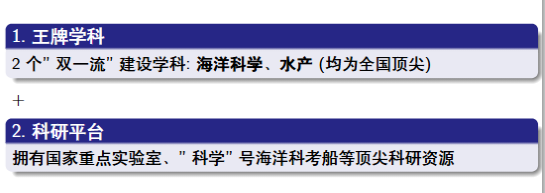
\includegraphics[width=0.8\textwidth]{1.png}
     \caption{}
     \end{figure}
\end{enumerate}
\subsection{git练习内容}
\begin{enumerate} 
    \item 查询最后修改了 README.md 文件的方法:使用 git log 命令并指定文件名。这个命令会显示该文件的所有提交记录,默认按时间倒序排列,因此最新的提交会显示在最前面。
    \item 查询最后一次修改config.yml文件中collections: 行时的提交信息是什么的方法:1.使用 git blame 定位具体行和提交哈希 2.从 git blame 的输出中提取提交哈希 (commit hash) 3.使用 git show 查看该次提交的详细信息
    \item 如何比较不同版本之间的差异?使用git diff:
    \item 如何初始化新仓库?
          git init,将当前目录变为 Git 仓库
    \item 如何克隆远程仓库? git clone <远程仓库地址>,将远程仓库复制到本地
    \item 如何添加文件到暂存区?使用git add <文件名> 或 git add.将工作区的改动添加到暂存区
    \item 如何如何提交更改?使用git commit -m 提交说明,将暂存区内容提交到本地仓库
    \item 如何查看状态?使用git status,查看工作区和暂存区状态
    \item 如何创建新分支?git branch <分支名>,基于当前分支创建一个新分支
    \item 如何切换到指定分支?git checkout <分支名>
    \item 如何拉取远程更新并合并?使用git pull origin <分支名>	获取远程分支最新内容并合并到当前本地分支
    \item 如何将本地分支的提交推送到远程仓库?git push origin<分支名>
\end{enumerate}
\section{练习结果}
\subsection{LaTeX}
\begin{itemize}
\item 成功使用 ctexart 文档类创建了中文文档
\item 使用了 titlesec, graphicx, indentfirst, hyperref 等宏包
\item 理解了 beamer 文档类中 frame, block, figure 环境的基本用法
\item 了解了 LaTeX 文档的基本结构(begin{document}...end{document})。
\end{itemize}

\subsection{Git}
\begin{itemize}
\item 掌握了使用 git log 查看指定文件提交历史的方法。
\item 掌握了使用 git log 查看指定文件提交历史的方法。
\item 练习了 Git 的基本工作流程:init -> add -> commit -> (branch/checkout) -> push/pull。
\item 理解了 .gitignore 文件的作用
\end{itemize}

\section{解题感悟}
\begin{enumerate}
    \item LaTeX 的文档结构(如 section{}, itemize, enumerate)强制逻辑清晰的方式对内容进行,避免了Word 排版中常见的格式错乱问题
    \item Git 不仅解决了写作中的版本回溯问题,如通过 git log 查看历史修改,还通过分支管理,如 git branch,进行多场景协作
\end{enumerate}

\end{document}




